\subsection{Address Translation Attacks}
\label{sec:address_translation_attacks}

\S~\ref{sec:system_software_attacks} argues that today's system software is
virtually guaranteed to have security vulnerabilities. This suggests that a
cautious secure architecture shoild avoid having the system software in the
TCB.

However, removing the system software from the TCB requires that the
architecture provides a method for isolating sensitive application code from
the untrusted system software. This is typically accomplished by a designing a
mechanism for loading application code in isolated containers whose contents
can be certified via software
attestation~(\S~\ref{sec:generic_software_attestation}). One of the more
difficult problems faced by these designes is that application software relies
on the memory management services provided by the system software, which is now
untrusted.

Intel's SGX~\cite{mckeen2013sgx, anati2013sgx}, leaves the system software in charge of
setting up the page tables (\S~\ref{sec:paging}) used by address translation, inspired by Bastion~\cite{champagne2010bastion},
but instantiates access checks that prevent the system software from directly
accessing the isolated container's memory.

This section discusses some attacks that become relevant when the application
software does not trust the system software which in charge of the page tables.
Understanding these attacks is a prerequisite to reasoning about the security
properties of architectures with this threat model. For example, a large amount
of the mechanisms in SGX are aimed at dealing with a subset of the attacks
described here.


\subsubsection{Passive Attacks}
\label{sec:fault_tracking_attacks}

System software uses the the CPU's address translation feature
(\S~\ref{sec:paging}) to implement page swapping, where infrequently used
memory pages are evicted from DRAM to a slower storage medium. Page swapping
relies the accessed (A) and dirty (D) page table entry attributes
(\S~\ref{sec:page_table_attributes}) to identify the DRAM pages to be evicted,
and on a page fault handler (\S~\ref{sec:faults}) to bring evicted pages back
into DRAM when they are accessed.

Unfortunately, the features that support efficient page swapping turn into a
security liability, when the system software managing the page tables is not
trusted by the application software using the page tables. The system software
can be prevented from reading the application's memory directly by placing the
application in an isolated container. However, potentially malicious system
software can still infer partial information about the application's memory
access patterns, by observing the application's page faults and page table
attributes.

We consider this class of attacks to be passive attacks that exploit the CPU's
address translation feature. It may seem that the page-level memory access
patterns provided by these attacks are not very useful. However,
\cite{xu2015pagefaults} describes how this attack can be carried out against
Intel's SGX, and implements the attack in a few practical settings. In one
scenario, which is particularly concerning for medical image processing,
the outline of a JPEG image is inferred while the image is decompressed inside
a container protected by SGX's isolation guarantees.


\subsubsection{Straightforward Active Attacks}
\label{sec:memory_mapping_attacks}

We define active address translation attacks to be the class of attacks where
malicious system software modifies the page tables used by an application in
a way that breaks the virtual memory abstraction (\S~\ref{sec:paging}). Memory
mapping attacks do not include scenarios where the system software breaks the
memory abstraction by directly writing to the application's memory pages.

We begin with an example of a straight-forward active attack. In this example,
the application inside a protected container performs a security check to
decide whether to disclose some sensitive information. Depending on the
security check's outcome, the enclave code either calls a \texttt{errorOut}
procedure, or a \texttt{disclose} procedure. The simplest vesion of the attack
assumes that each procedure's code starts at a page boundary, and takes up less
than a page. These assumptions are relaxed in more complex versions of the
attack.

In the most straightforward setting, the malicious system software directly
modifies the page tables of the application inside the container, as shown in
Figure~\ref{fig:active_mapping_attack}, so the virtual address intended to
store the \texttt{errorOut} procedure is actually mapped to a DRAM page that
contains the \texttt{disclose} procedure. Without any security measures in
place, when the application's code jumps to the virtual address of the
\texttt{errorOut} procedure, the CPU will execute the code of the
\texttt{disclose} procedure instead.

\begin{figure}[hbt]
  \centering
  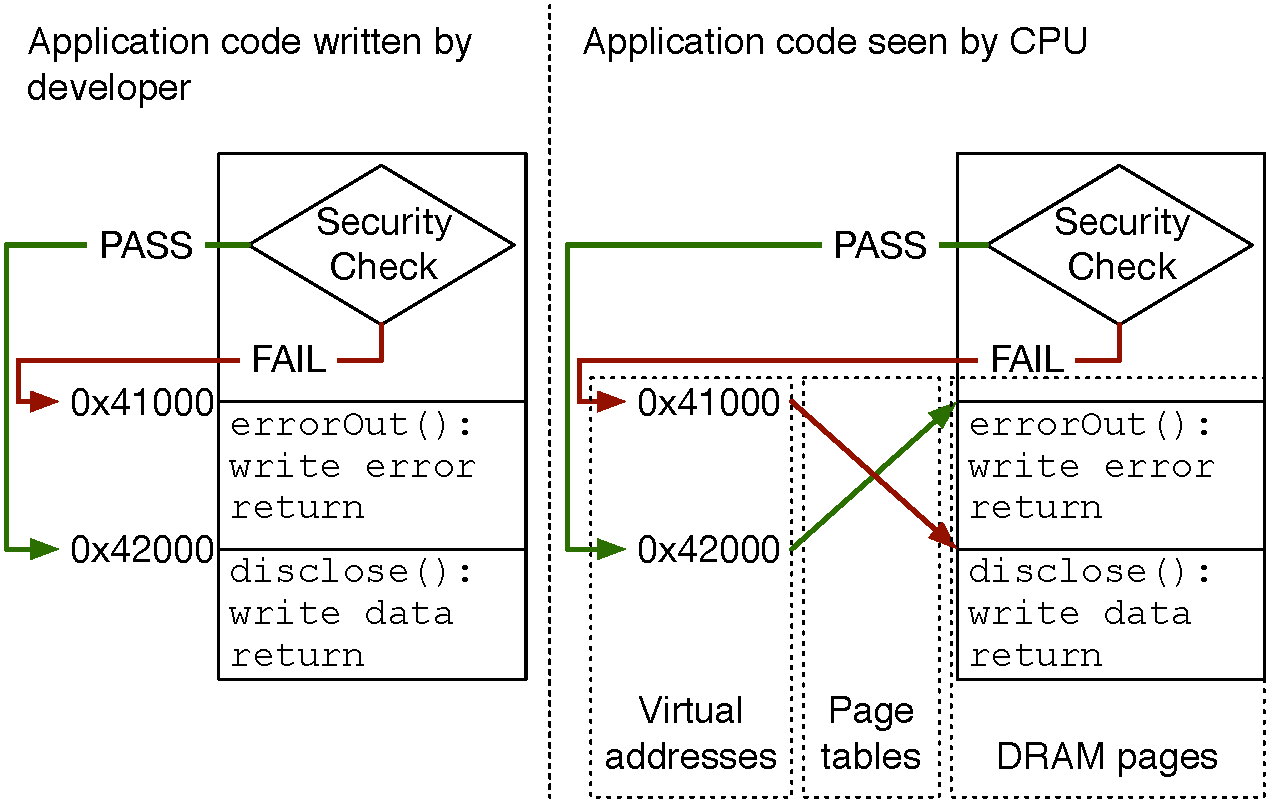
\includegraphics[width=85mm]{figures/active_mapping_attack.pdf}
  \caption{
    An example of an active memory mapping attack. The application's author
    intends to peform a security check, and only disclose a piece of sensitive
    information if the check passes. Malicious system software maps the virtual
    address of the procedure called when the security check fails to a DRAM
    page that contains the procedure that discloses the sensitive information,
    which is supposed to be called when the security check passes.
  }
  \label{fig:active_mapping_attack}
\end{figure}


\subsubsection{Active Attacks Using Page Swapping}
\label{sec:page_swapping_attacks}

The most obvious active attacks on memory mapping can be defeated by tracking
the correct virtual address for each DRAM page that belongs to a protected
container. However, a naive protection measure based on address tracking can be
defeated by a more subtle active attack that relies on the architectural
support for page swapping. Figure~\ref{fig:swap_mapping_attack} illustrates an
attack that does not modify the application's page tables, but produces the
same corrputed CPU view of the application as the straight-forward attack
described above.

\begin{figure}[hbt]
  \centering
  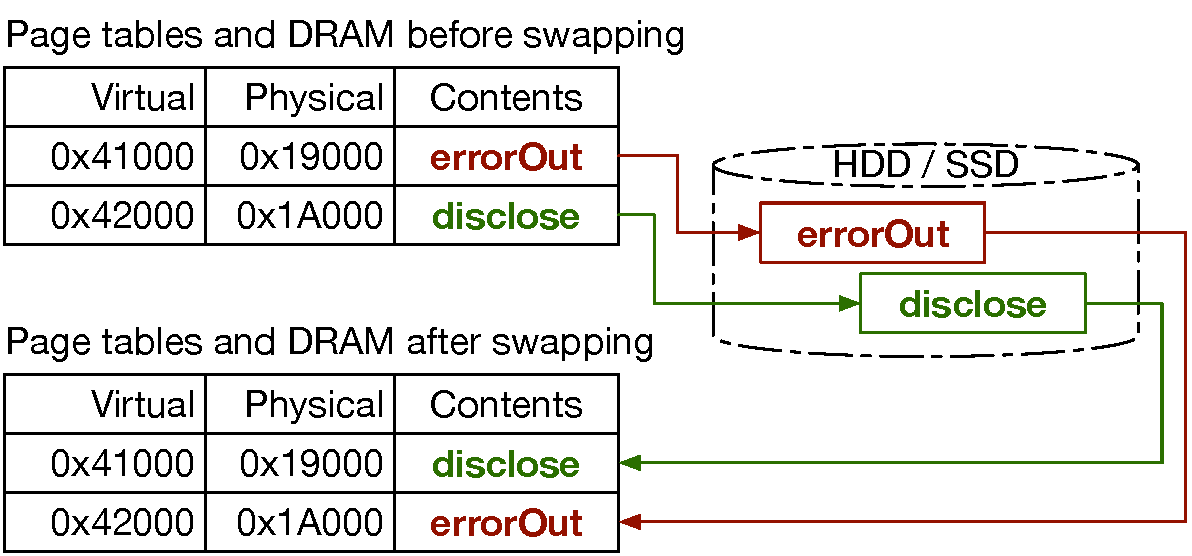
\includegraphics[width=85mm]{figures/swap_mapping_attack.pdf}
  \caption{
    An active memory mapping attack where the system software does not modify
    the page tables. Instead, two pages are evicted from DRAM to a slower
    storage medium. The malicious system software swaps the two pages' contents
    then brings them back into DRAM, building the same incorrect page mapping
    as the direct attack shown in Figure~\ref{fig:active_mapping_attack}. This
    attack defeats protection measures that rely on tracking the virtual and
    disk addresses for DRAM pages.
  }
  \label{fig:swap_mapping_attack}
\end{figure}

In the swapping attack, malicious system software evicts the pages that contain
the \texttt{errorOut} and \texttt{disclose} procedures from DRAM to a slower
medium, such as a hard disk. The system software exchanges the hard disk
bytes storing the two pages, and then brings the two pages back into DRAM.
Remarkably, all the steps taken by this attack are indistinguishable from
legitimate page swapping activity, with the exception of the I/O operations
that exchange the disk bytes that store evicted pages.

The subtle attack described in this section can be defeated by
cryptographically binding the contents of each page that is evicted from DRAM
to the virtual address that the page should be mapped to. The cryptographic
primitive (\S~\ref{sec:crypto_primitives}) used to perform the binding must
obiously guarantee integrity. Furthermore, it must also guarantee freshness, in
order to foil replay attacks where the system software ``undoes'' an
application's writes by evicting one of its DRAM pages to disk and bringing in
an older version of the same page.


\subsubsection{Active Attacks Based on TLBs}
\label{sec:tlb_mapping_attacks}

Today's multi-core architectures can be subjected to an even more subtle active
attack, illustrated in Figure~\ref{fig:tlb_mapping_attack}, which can bypass
any protection measures that solely focus on the integrity of the page tables.

\begin{figure}[hbt]
  \centering
  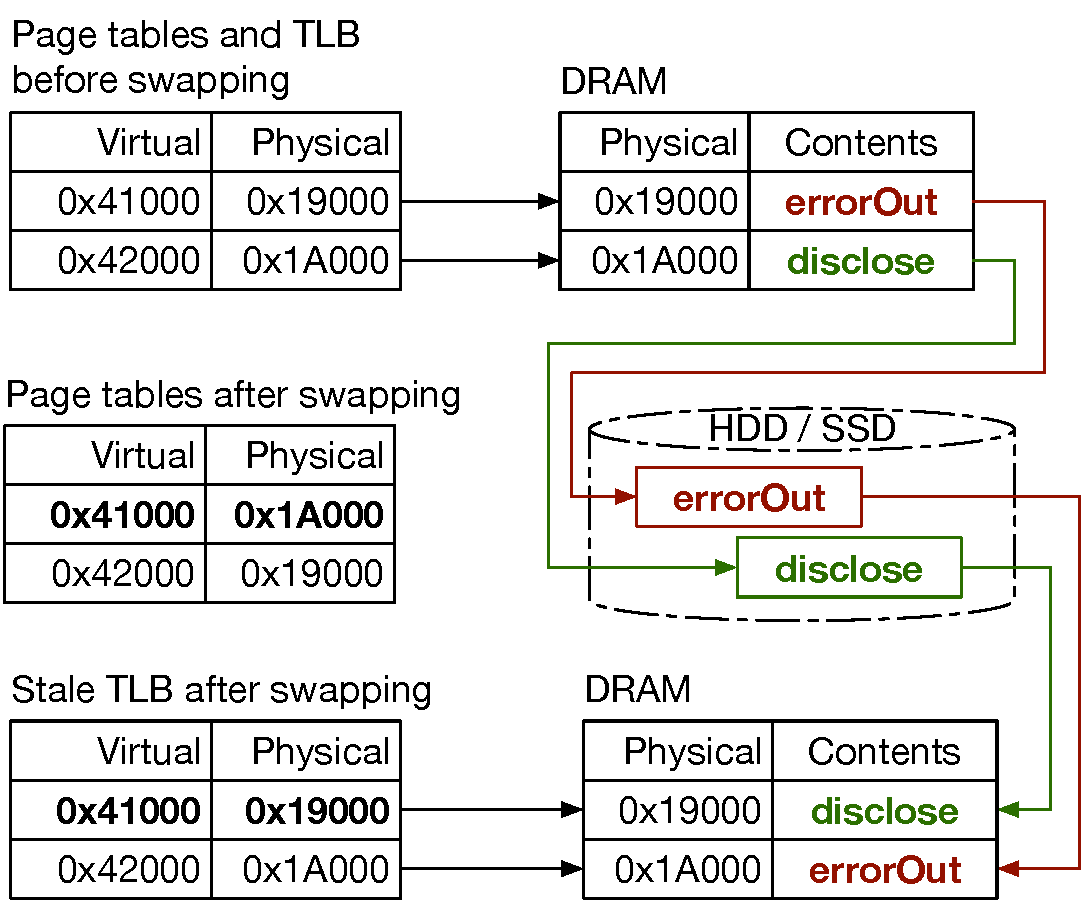
\includegraphics[width=75mm]{figures/tlb_mapping_attack.pdf}
  \caption{
    An active memory mapping attack where the system software does not
    invalidate a core's TLBs when it evicts two pages from DRAM and exchanges
    their locations when reading them back in. The page tables are updated
    correctly, but the core with stale TLB entries has the same incorrect view
    of the protected container's code as in
    Figure~\ref{fig:active_mapping_attack}.
  }
  \label{fig:tlb_mapping_attack}
\end{figure}

For performance reasons, each execution core caches address translation results
in its own translation look-aside buffer~(TLB,~\S~\ref{sec:tlbs}). For
simplicity, the TLBs are not covered by the cache coherence protocol that
synchronizes data caches across cores. Instead, the system software is
responsible for invalidating TLB entries across all the cores when it modifies
the page tables.

Malicious system software can take advantage of the design decisions explained
above by carring out the following attack. While the same software used in the
previous examples is executing on a core, the system software executes on a
different core and evicts the \texttt{errorOut} and \texttt{disclose} pages
from DRAM. Like in the previous attack, the system software loads the
\texttt{disclose} code in the DRAM page that previously held \texttt{errorOut}.
In this attack, however, the system software also updates the page tables.

The core where the system software executed sees the code that the application
developer intended. Therefore, the attack will pass any security checks that
rely cryptographic associations between page contents and page table data, as
long as the checks are performed by the core used to load pages back into DRAM.
However, the core that executes the protected container's code still uses the
old page table data, because the system software did not invalidate its TLB
entries. Assuming the TLBs are not subjected to any additional security checks,
this attack causes the same private information leak as the previous examples.

In order to avoid the attack described in this section, the trusted software or
hardware that implements protected containers must also ensure that the system
software invalidates the relevant TLB entries on all the cores when it evicts a
page from a protected container to DRAM.
